\chapter{绪论}
\thispagestyle{others}
\pagestyle{others}
\xiaosi

\section{研究背景及意义}
近些年来,计算机视觉的发展让我们的生活越来越便利。与此同时,随着我国信息化水平和自动化进程的不断提高与推进,国家对计算机视觉的应用和发展也提出了更高要求。相比于二维图像,三维点云数据能更加清晰的表示我们所处的三维世界。图\ref*{fig:1-1}显示了两对激光雷达点云和图像的例子,它们分别取自于不同时间的同一场景。可以清晰的观察到,点云的几何结构在光照和季节变化的情况下能够保持基本不变,而图像的变化使得人眼也难以分辨出这对图像来自于同一场景。由于点云数据具有光照不变性,能够有效避免图像处理过程中的问题,因此越来越多的研究人员开始研究点云并从中获益。但是三维视觉传感器的视野范围是有限的,因此为了感知全局的环境,在应用中经常需要将若干不同位置采集的点云数据对齐到世界坐标系下。因此,点云配准已成为许多任务的基础问题,近年来备受关注。

\vspace{-0.1cm}
\begin{figure}[h]
    \centering 
    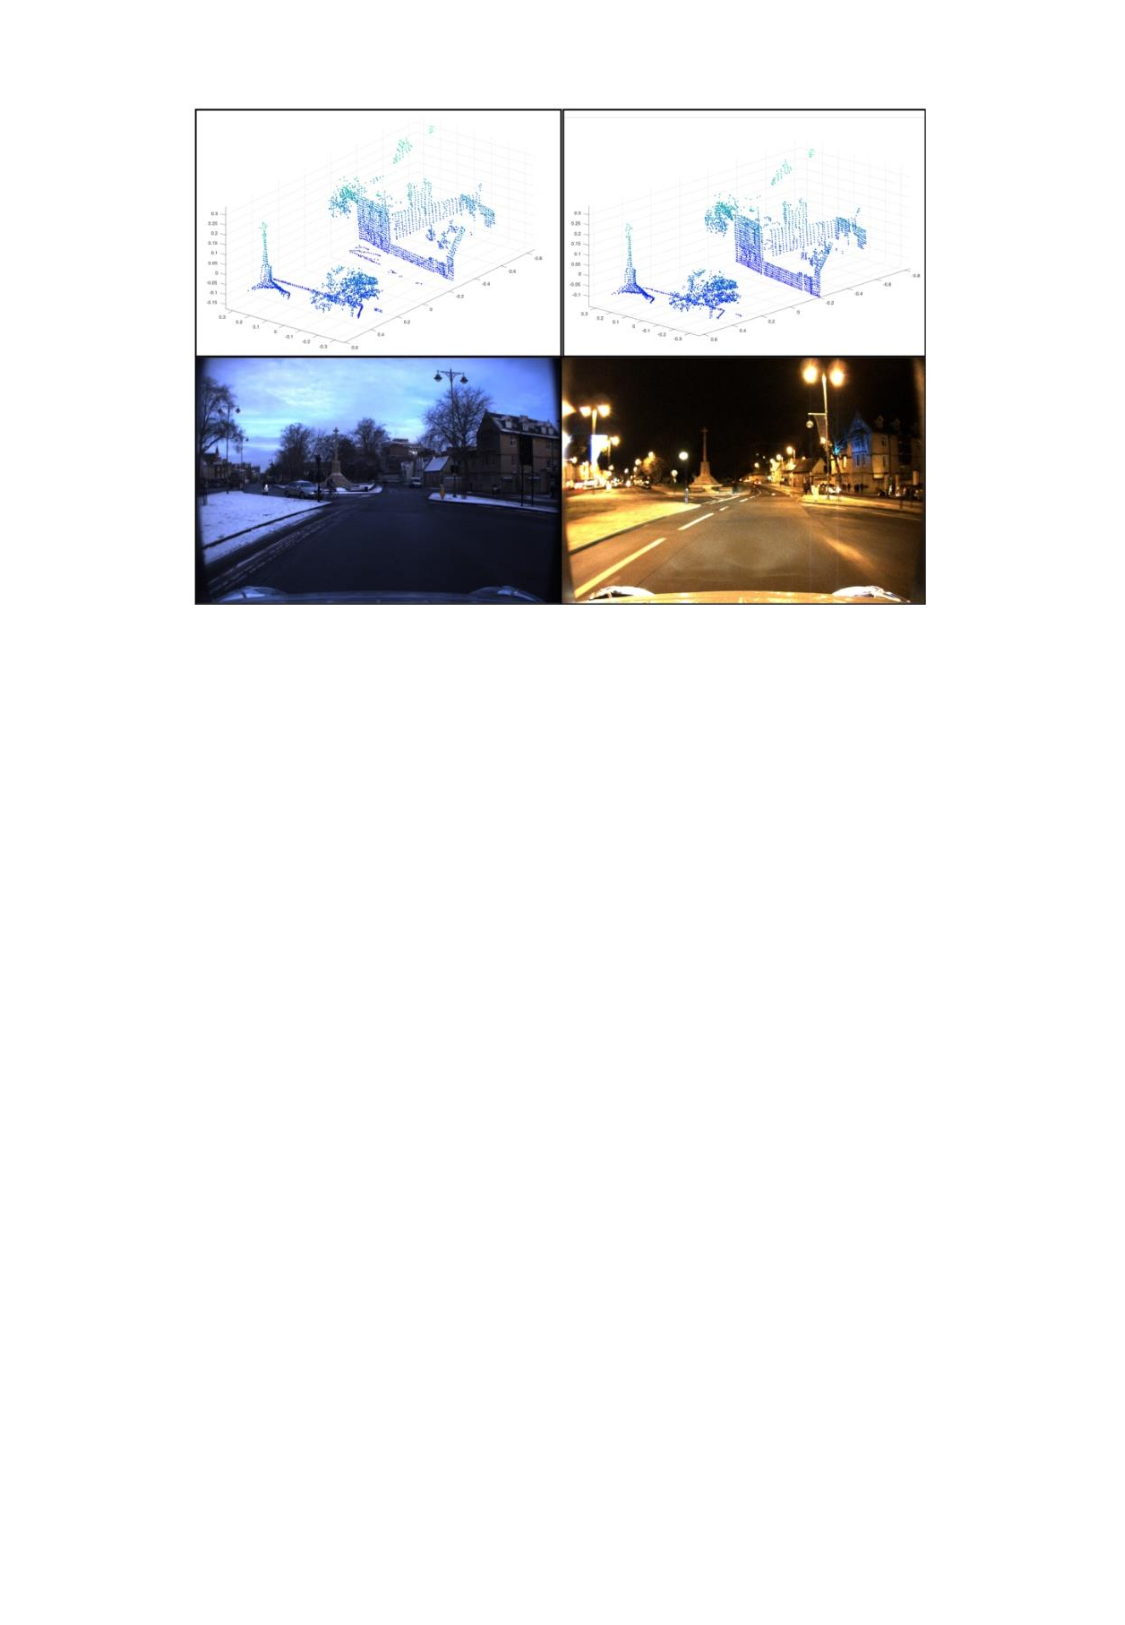
\includegraphics[width=\textwidth]{my/figure/1-1.pdf}
    \bicaption[\xiaosi 不同时间同一场景的点云与图像对比]
    {\wuhao 不同时间同一场景的点云与图像对比\upcite{PointNetVLAD}}
    {\wuhao Comparison between point cloud and image of the same scene at different time\upcite{PointNetVLAD}}
    \label{fig:1-1} 
\end{figure}
\vspace{-0.35cm}

在医疗领域,使用点云配准能够将患者的器官及内脏等组织融合成一个整体构建三维模型,辅助医生诊断。在文物修复领域,研究人员能过够对大型文物多次扫描后将其配准生成完整的文物模型,不仅能够存储文物的三维数据以实现文物的数字化存储,还能够为后续文物的保护和修复提供可靠的数据\upcite{文物}。在工业领域,点云配准是逆向工程的重要一环,能够为研究人员提供产品模型的三维数据\upcite{逆向工程}。更重要的是,点云配准是许多机器人任务的关键组成部分,是机器人对环境感知的重要一环\upcite{Map-matching}。在同时定位与建图(Simultaneous Localization And Mapping,SLAM)中,点云配准可以构建用于自动驾驶的路径规划和决策的三维地图\upcite{LCDNet}。点云配准也广泛应用于位置识别,它能够将实时的三维视图匹配到所属的三维地图中,以实现机器人对自身位置的定位\upcite{LPD}。同时点云配准在机器人的姿态估计中也发挥着不可或缺的作用。通过对齐视图与环境,可以获取机器人手臂的姿态信息,进而决定下一步该如何移动以抓取物体\upcite{2015review}。

点云配准是三维图形学研究的一个重要研究课题,也是计算机视觉的重要分支,其目的是将两个具有部分重叠区域的点云,经过一个变换矩阵在同一个坐标系下对齐。早期,不少学者提出了许多不同的方法来解决点云配准问题,这些方法主要针对于实验室理想环境下的合成数据集,而这些数据集也往往由单一的物体模型而不是场景构成。随着社会的发展,这些方法已经不能够满足生产生活需要。近年来越来越多的工作开始关注真实环境下的点云配准,其中基于深度学习的点云配准方法有着突出的表现。最近,针对低重叠率情况的点云配准得到了学界的广泛关注。所谓低重叠率的点云配准指的是将两个至多只存在30\%重叠区域的点云进行对齐。相比于一般情况的点云配准,低重叠率的点云对之间存在许多相似非重叠区域,这会很大程度上增加特征搜索寻找正确点对应的难度,导致大量非匹配区域的误匹配。由此可见低重叠情况下的点云配准的研究重点在于如何将点的对应关系聚集在重叠区域和如何增加相似区域的特征差异。

综上所述,点云配准是处理点云数据的一项基本任务,是推进自动化进程的关键一环,在生产生活中扮演着重要的角色。因此,研究点云配准算法,提高配准精度和减少算法时间复杂度具有重大的研究价值。同时,随着近年来人工智能深度学习的快速发展,基于深度学习的点云配准方法也取得了巨大成功。本文通过对现有方法研究进行分析并改进,提高在低重叠度的情况下点云配准算法的成功率。
% 由于传感器的视野有限,单次扫描只能捕捉一定空间的信息。因此将两个点云对齐的点云配准算法是正确处理点云数据基础。在点云配准中有两个相互关联的子问题:找到使两个点云对齐的刚性变换和找到两个点云之间点对点的对应关系。虽然在已知其中某个子问题的解时,另一个子问题很容易求解,但要同时求解两个子问题是比较困难的。尤其存在异常值时,点云配准将变得更加困难。其中异常值是指部分点在另一个点云中没有对应的点。异常值可能来自于用于收集点云的传感器的不完善或两个要配准的点云没有完全重叠的情况。

\section{国内外研究现状}
本节将从传统点云配准方法和基于深度学习的点云配准方法两个方向介绍点云配准方法的研究现状。其中传统点云配准方法早在上世纪90年代就得到了初步发展,而后在研究人员的不懈努力下传统方法的点云配准现在已经广泛应用于工业生产领域。随着近些年来的人工智能的发展,将点云配准与与深度学习融合也逐渐受到越来越多的研究人员的关注,并且其性能上已经超过传统的点云配准方法。

    \subsection{传统点云配准方法}
    迭代式最近点法\upcite{ICP}(Iterative Closet Points,ICP)是传统点云配准方法中最典型的一类,它由BESL等人在1992年提出。ICP方法通过计算源点云和目标点云原始点之间的欧氏距离,以最临近点作为对应点确定两点云间点的对应关系。然后,在已知点的对应关系时,通过基于奇异值分解法求解两点云之间的变换矩阵,并进行单次对齐。重复上述两个步骤直至满足预设要求完成整个配准过程。当源点云与目标点云之间具有良好的初始位姿时,ICP方法可以取得良好的配准结果。但是,当二者之间的距离较大时,该算法往往会在局部最优点处收敛,导致最终的结果不能满足实际生产生活需要。文献\cite{1998}提出一种模拟退火算法将ICP算法中根据点到点的距离确定的“硬”匹配关系转化为一种“软”匹配方式。这种方法虽然不能完全避免局部最优解问题,但是能够使算法在一定程度上得到缓解。YANG等人\upcite{Go-ICP}为了解决上述问题,提出一种全局最优的迭代式最近点算法(Globally Optimal Iterative Closet Point, Go-ICP),其基本思想是通过分支界定法跳出局部最优解,以实现全局最优解,但与此同时算法的速度严重下降。

    基于图的配准是另一类常见的方法,它主要是寻找更加准确的对应关系。相比于ICP方法中直接选取最邻近点作为对应点,基于图的配准方法将同时考虑点和边的关系。具体而言,图匹配算法不仅要求匹配点的点相似度高,而且要求节点之间的连线即边的相似度也要高。这种关系能够找到更准确的对应关系,而精确的对应关系有助于更好的变换估计。图匹配的优化属于二次分配问题,是一个典型的NP难问题,解决思想主要采取近似策略逼近。文献\cite{Almohamad}和文献\cite{CSGM}采用线性规划来解决图匹配问题。文献\cite{FGM}则将较大的相似矩阵分解为若干较小矩阵,这些矩阵对每个图的局部结构和相似性进行编码,解耦节点和边之间的相似性,使得求解过程简化。LERDEANU等人\upcite{Leordeanu}提出了一种谱松驰的方法来近似二次分配问题,它指出正确的对应能够形成强关联的集群,而错误的对应只是一种偶然,因此不太可能产生强关联的簇,根据这一特性能够有效找出正确的对应关系。

    高斯混合模型(Gaussian Mixture Models, GMM)是另一种常见的点云配准方法,它的核心思想是将配准问题中变换估计问题转化为求解点云数据的最大似然估计问题。任意两点之间的对应关系,将由原来的“硬”匹配转化为了由置信度表示的“软”匹配,但也因此其时间复杂度大大增加了。JRMPC等人\upcite{JRMPC}提出了一个EM算法,它估计了GMM参数以及将每个独立集合映射到“中心”模型上的旋转和平移。文献\cite{CPD}通过最大似然估将源点云数据拟合到目标点云。使源点云作为一个整体移动,以保持点集的拓扑结构。通过对具有刚性参数的GMM质心位置的重新参数化来施加一致性约束,并推导出EM算法的最大步骤的封闭解。文献\cite{CH-GMM}提出了一种新的凸包索引高斯混合模型。该模型通过计算每个点集凸包上的加权高斯混合模型响应来工作。

    传统的点云配准算法的优点有两个方面:(1)严格的数学理论可以保证算法的收敛性;(2)不需要训练数据。然而这类方法的局限性也较为明显:ICP算法需要一个较好的初始位置才能有良好的表现,这在真实场景下尤其是低重叠情况下难以达到要求;这类方法对数据的离群值、噪声和点云密度等特点较为敏感,在真实场景下的表现远没有在合成数据上的表现好。

    \subsection{基于深度学习的点云配准方法}
    基于深度学习的点云配准方法大致可以分为两类:端到端的点云配准方法和基于对应关系的点云配准方法。\par
    \subsubsection{端到端的点云配准方法}
    文献\cite{PointNetLK}提出的PointNetLK可以被认为是一个可学习的函数。因此,将用于图像对齐的经典视觉算法Lucas-Kanade\upcite{LucasKanade}(LK)算法与其相结合,并融合为一个循环深度神经网络。
    文献\cite{PPF}赋予PPF-FoldNet自动编码器(Auto Encoder,AE)一个姿态差异结构,其中两者之间的差异产生特定于姿态的描述符。在此基础上,引入了相对姿态估计网络RelativeNet,为关键点分配对应特定的方向。最后,利用一个简单而有效的假设-验证算法来快速预测和对齐两个点云。
    % 文献\cite{PCRNet}提出了PCRNet用来比较源点云和目标点云的全局特征。根据点云的物体形状的先验信息,生成特定形状包括不可见的形状,并使用带有全连接层的暹罗架构增加网络的鲁棒性。
    FMR\upcite{FMR}借鉴了PointNetLK的思想,利用刚性变换的可逆特性,采用编解码器结构监督全局特征。
    文献\cite{OMNet}提出了一种基于全局特征的迭代网络OMNet,用于部分重叠点云的配准。OMNet以由粗到细的方式学习掩码来拒绝非重叠区域,这将部分重叠的配准转换为相同形状的配准。此外,它提出了一种更实用的数据生成方式,其中CAD模型对源点云和参考点云进行两次采样,避免了普遍存在的过拟合问题。
    \vspace{-0.1cm}
    \begin{figure}[h]
        \centering 
        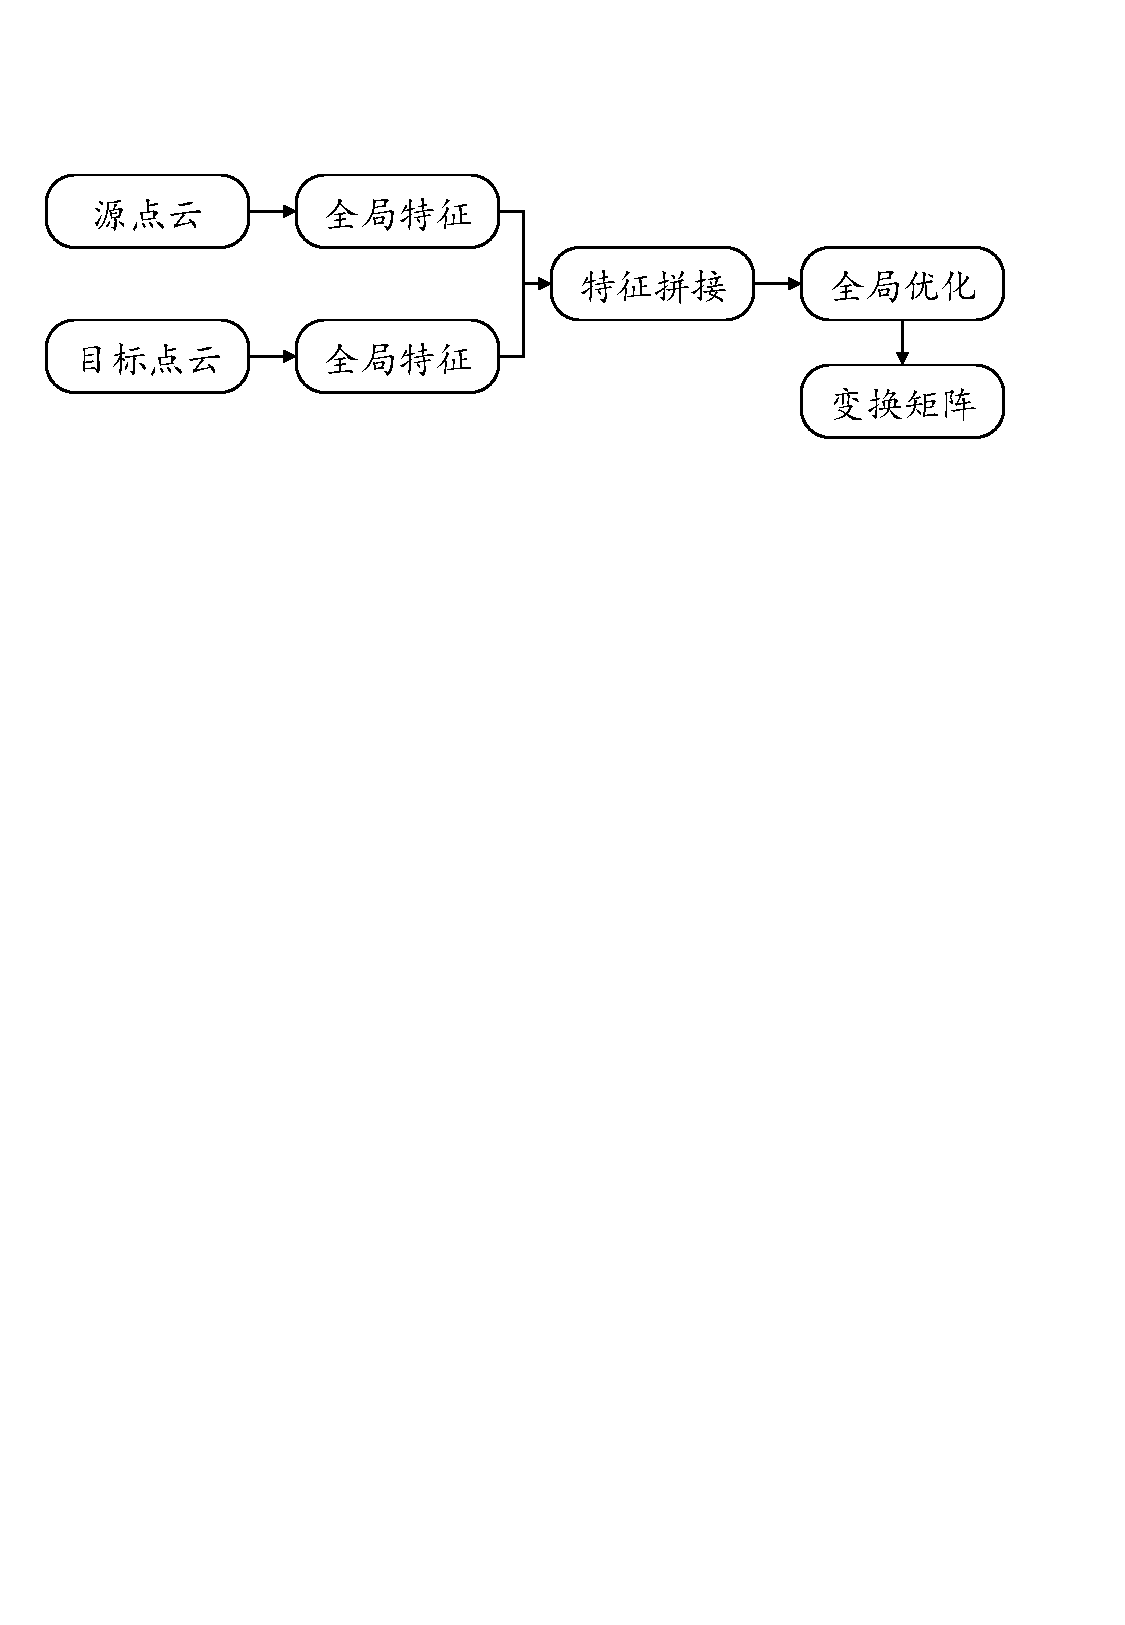
\includegraphics[width=12cm]{my/figure/1-2.pdf}
        \bicaption[\xiaosi 端到端的点云配准方法流程图]{\wuhao 端到端的点云配准方法流程图}{\wuhao Flowchart of the end-to-end point cloud registration}
        \label{fig:1-2} 
    \end{figure}
    \vspace{-0.2cm}
    % Deng等人将PPF特征和点云分别输入到PPF-foldnet和PC-FoldNet网络中,得到包含结构和姿态的新特征,并使用RelativeNet预测相对姿态。
    % PCRNet在拼接两个点云的全局特征后,使用类似于Siamese的网络来预测变换矩阵。FMR借鉴了PointNetLK的思想,利用刚性变换的可逆特性,采用编解码器结构监督全局特征。
    % Xu等人提出OMNet在迭代过程中预测源点云和目标点云的重叠掩码,通过mlp从两者的全局特征预测刚性转换。然而,直接配准方法在处理真实场景时往往受到限制。

    \subsubsection{基于对应关系的点云配准方法}
    基于对应关系的配准方法主要集中在四个方面:特征提取、关键点检测、异常值去除和位姿估计。
    QI等人先后提出了PointNet\upcite{PointNet}和pointnet++\upcite{PointNet++}。这两种方法虽然为点云的特征提取提供了参考,但都没有考虑点云的几何结构特征。
    文献\cite{3DFeat-Net}提出了一种利用弱监督学习三维特征检测器和描述子进行点云匹配的3DFeat-Net。与许多以往的工作不同,该方法不需要手动标注匹配的点。相反,可以利用对齐和注意力机制从全球定位系统(Global Positioning System,GPS)标记的3D点云中学习特征对应关系,而无需人工标注。
    文献\cite{PerfectMatch}提出了3DSmoothNet,它利用暹罗网络架构匹配3D点云,并使用体素化平滑密度值表示实现全卷积层,并与局部参考系对齐以实现旋转不变性。
    文献\cite{DGCNN}提出了一种新的神经网络模块EdgeConv,构造了DGCNN来捕获点之间的拓扑信息。EdgeConv作用于网络每一层中动态计算的图,其中包含了局部邻域信息,并可以叠加应用于学习全局形状属性。
    文献\cite{KPConv}提出KPConv来模拟二维卷积中的运算,以更好地捕获局部几何信息。
    文献\cite{3DMatch}提出的3DMatch网络以体素为输入,利用三维卷积神经网络学习局部几何特征。
    文献\cite{FCGF}提出全卷积几何特征采用稀疏三维卷积代替传统的三维卷积来缓解点云稀疏性带来的问题。
    SpinNet\upcite{SpinNet}通过估计的参考轴约束z轴自由度,并使用球面体素化消除XY平面旋转自由度,提取具有高鲁棒性的特征。
    文献\cite{D3Feat}提出的D3feat在提取点云特征时使用KPConv组成的U-Net网络来检测关键点,并使用密度不变显著性评分来缓解密度对显著性的影响。
    文献\cite{PREDATOR}提出了一种点云配准模型Predator,该模型对重叠区域进行了深度关注。与以前的工作不同,该模型是专门设计来处理低重叠的点云对的。其核心思想是在两个点云的潜在编码之间进行早期信息交换的重叠注意块,以预测哪些点不仅是显著的,而且还位于两个点云之间的重叠区域。
    
    \vspace{-0.1cm}
    \begin{figure}[h]
        \centering 
        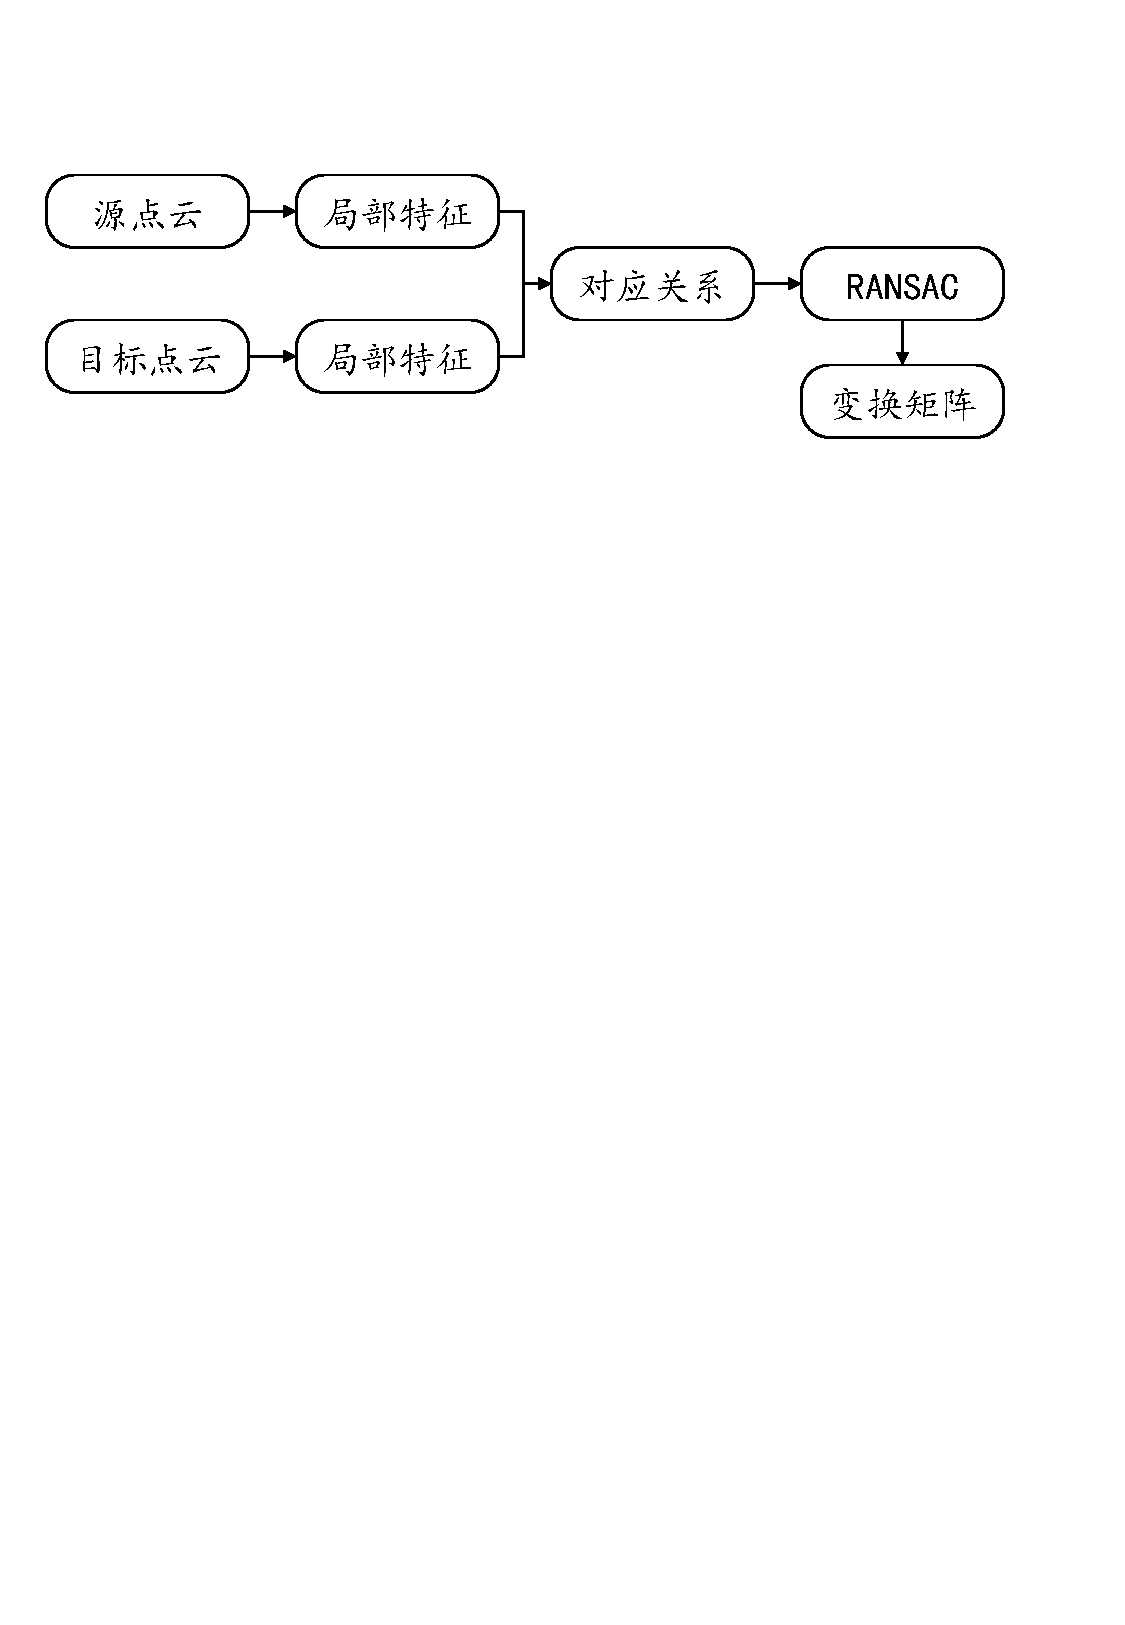
\includegraphics[width=12cm]{my/figure/1-3.pdf}
        \bicaption[\xiaosi 基于对应关系的点云配准方法流程图]{\wuhao 基于对应关系的点云配准方法流程图}{\wuhao Flowchart of point cloud registration method based on correspondence}
        \label{fig:1-3} 
    \end{figure}
    \vspace{-0.35cm}

    文献\cite{PointDSC}提出PointDSC,将传统方法中的空间几何一致性约束添加到网络中,利用神经网络提取对应关系的特征,通过可微的光谱匹配模块,对成对的空间一致性监督,以估计每个对应的嵌入特征的置信度。
    文献\cite{DCP}提出一个由点云嵌入网络、结合注意力模块近似组合匹配层、可微奇异值分解层三部分组成的DCP网络,解决局部最优和ICP方法中的其他问题。
    IDAM\upcite{IDAM}包括一个迭代的距离感知相似矩阵卷积模块,将来自特征和欧几里得空间的信息合并到成对点匹配过程中。这些卷积层学习基于整个几何特征的联合信息和每个点对的欧几里得偏移来匹配点,克服了通过简单地使用特征向量的内积来匹配的缺点。
    文献\cite{DGR}提出了一个可微分的框架DGR。它由三个模块组成:用于对应置信度预测的6维卷积网络,用于封闭姿态估计的可微分加权Procrustes算法,以及用于姿态细化的鲁棒基于梯度的SE(3)优化器。
    % \vspace{-0.1cm}
    % \begin{figure}[h]
    %     \centering 
    %     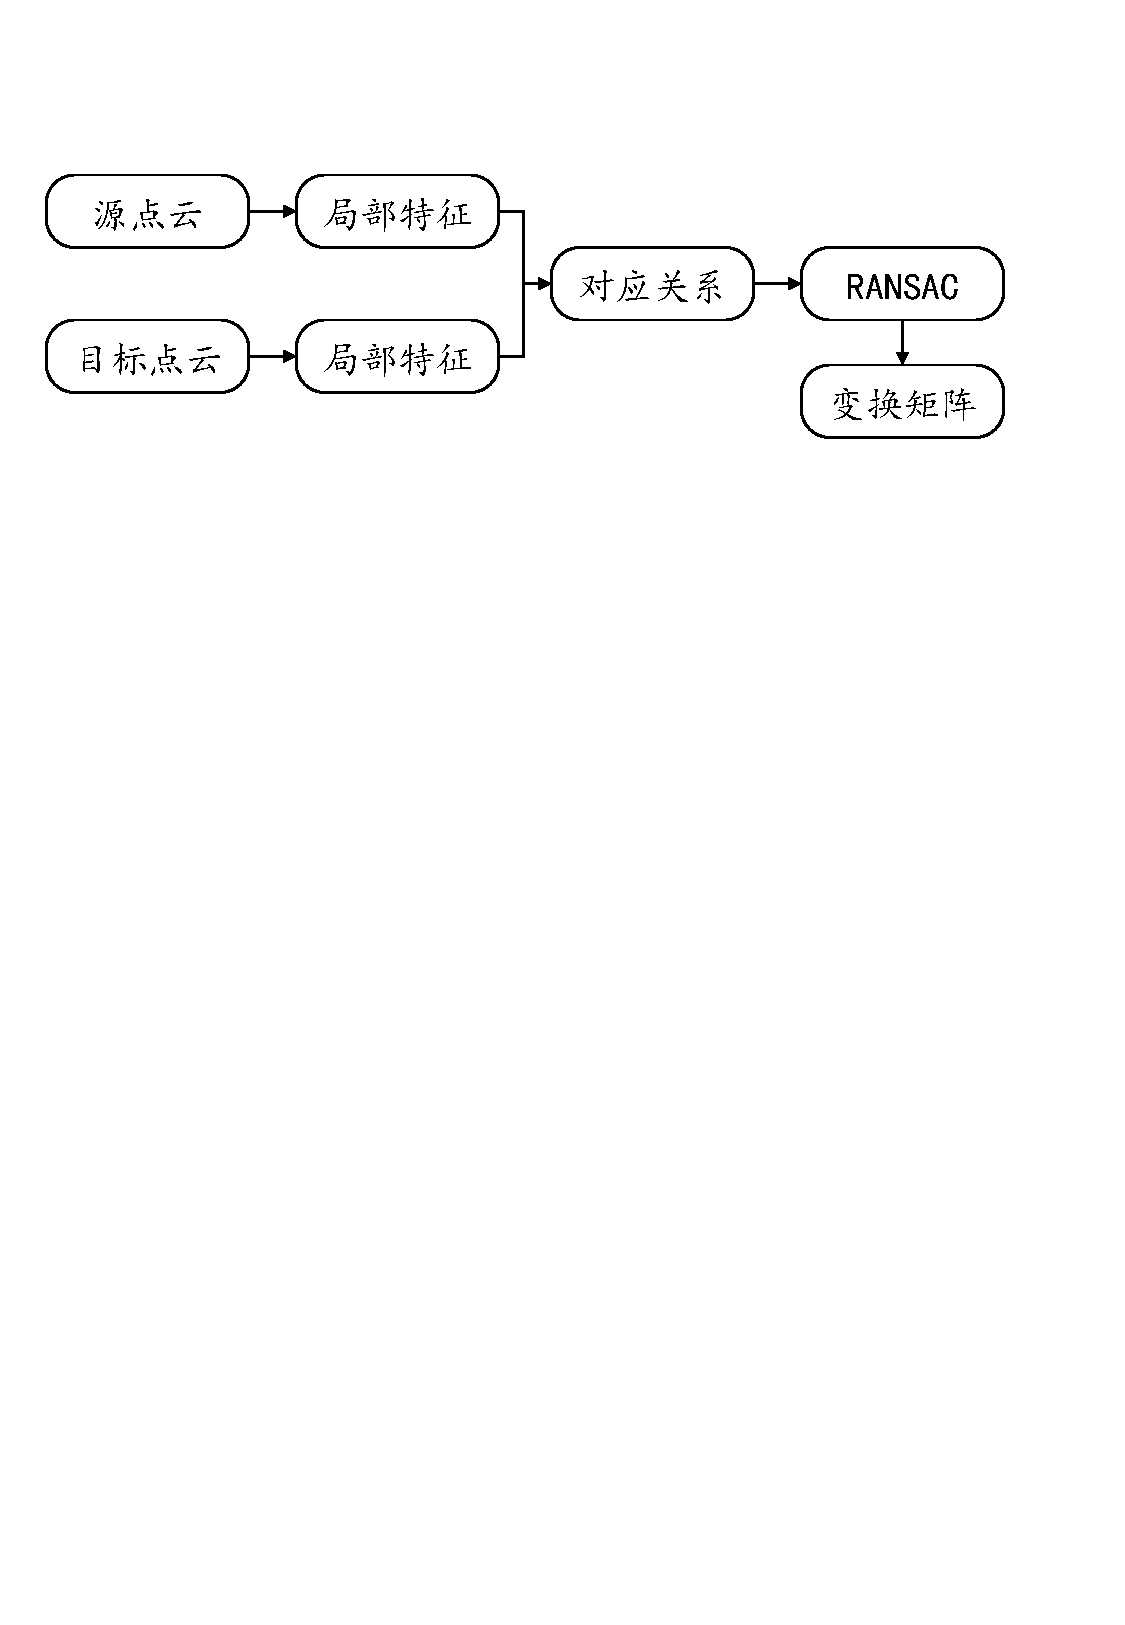
\includegraphics[width=12cm]{my/figure/1-3.pdf}
    %     \bicaption[\xiaosi 基于对应关系的点云配准方法流程图]{\wuhao 基于对应关系的点云配准方法流程图}{\wuhao Flowchart of point cloud registration method based on correspondence}
    %     \label{fig:1-3} 
    % \end{figure}
    % \vspace{-0.35cm}
    % Deng等人提出PPFNet,将点对特征(PPF)与点网相结合,提高了特征对噪声的鲁棒性。
    % Yew和Lee等人提出的3DFeatNet利用弱监督深度网络解决了点云数据精确标注的难题,提高了特征质量。
    % Gojcic等人提出了3DSmoothNet,它利用暹罗网络架构来编码光滑密度值体素化。
    % Wang等人设计了边缘卷积(EdgeConv)运算,构造了DGCNN来捕获点之间的拓扑信息。
    % Thomas等人提出KPConv来模拟二维卷积中的运算,以更好地捕获局部几何信息。
    % Zeng等人提出的3DMatch网络以体素为输入,利用三维卷积神经网络学习局部几何特征。
    % Choy等人提出FCGF采用稀疏三维卷积代替传统的三维卷积来缓解点云稀疏性带来的问题。
    % SpinNet通过估计的参考轴约束z轴自由度,并使用球面体素化消除XY平面旋转自由度,提取具有高鲁棒性的特征。
    % Bai等人提出的D3feat在提取点云特征时使用KPConv组成的U-Net网络来检测关键点,并使用密度不变显著性评分来缓解密度对显著性的影响。
    % Huang等在将任务扩展到低重叠场景的同时,通过检测重叠区域中点的可能性,提高了正确检测的概率。
    % Bai等提出PointDSC,将传统方法中的空间几何一致性约束添加到网络中,利用神经网络提取对应关系的特征,选择一组空间一致的点对。
    % DCP(深度最近点)和DeepVCP采用加权置信度估计相对位姿。
    % IDAM(迭代距离感知相似矩阵)和DGR(深度全局配准)通过选择高置信度点对,采用加权SVD求解刚性变换。
    \subsection{存在的问题}
    点云配准方法的研究已经有了二十多年的发展并且取得了一系列的成就,特别是在深度学习流行起来之后,许多研究利用深度神经网络取得了不错的成果。然而,在最近的相关文献\cite{Dope}中已经提到这些基于深度学习的方法的主干网络往往会遇到高层特征的过度平滑和结构模糊性相关的难以区分的特征问题,这是点云配准的一个关键瓶颈。它们忽略了特征提取的一个关键因素,这可能严重影响配准精度:源点云和目标点云中每个点特征的独特性;也就是说,为了获得精确的点对应关系,以估计最优刚性变换,所需的点特征应该充分表示任何给定点附近的几何模式,同时仍然与同一点云中围绕其它点的局部结构特征有足够的差异性。然而,许多工作\upcite{Deeper,Measuring}使用的骨干网络容易导致特征的超平滑和结构性的模糊问题,导致点特征难以区分。同时,将图像数据中的颜色和纹理信息引入进来通过多模态的融合,增加点特征之间的差异性是一个简单有效的想法。但是在相关研究中,许多多模态融合的方法并没有显示出比单模态的方法更加优异的表现。如何更有效的融合点云和图像两种模态的特征也是一个值得研究的问题。

\section{论文研究的主要内容}
本研究分别从嵌入几何结构和多模态融合两个方面入手,提高特征间的差异性,提出如下两个点云配准的方法。\par
1.基于显著锚点几何嵌入的点云配准方法。首先使用共享参数的骨干网络来提取源点云和目标点云的局部特征,在特征提取过程中同时对点云下采样进行超点聚合。之后在超点层面选取出若干分布于重叠区域的特征显著的锚点。同时,提出了一种新颖的基于注意力机制的几何嵌入方法。它的核心思想是将每个超点与锚点间的距离与角度信息进行编码,由于选取的多个锚点在空间中保持了一定的几何结构,因而使得这些超点与锚点之间的几何编码能够给每个超点带来各不相同的差异性特征。然后通过一个迭代优化模块,选取出更加显著的锚点进一步作结构嵌入增加特征差异性,并形成最终的超点对应。这些超点在物理空间中表示一个连续空间的区域,通过上采样能够建立超点与原始点之间的包含关系。这种由粗到细的配准方法可以在对应区域内部寻找点的对应关系而无需在全局点云中寻找,能够有效缓解特征平滑带来的误匹配,进而在变换估计中产生更加准确的变换矩阵。\par
2.基于多模态特征融合的锚点定位点云配准方法。现有的点云和图像两种模态融合方法往往通过对图像进行特征提取之后,将其与点云进行简单拼接并送入神经网络完成特征融合。与这些方法不同的是,本方法采用一种对齐策略,利用相机参数将点云和图像完成点与像素的对齐之后分别提取点云特征和图像特征。并利用点与像素之间的对应关系,通过交叉注意力机制完成像素到点的选择性融合。在此过程中,两种模态的特征均会被映射至模态无关与模态相关的两个特征子空间。在模态无关子空间中,点云和图像完成模态间特征的融合,随后将融合后的特征与点云在模态相关子空间中的投影相融合。这种方法能够有效减少点云和图像之间的域间隙,使得融合过程既不过多的引入噪声也不丢失互补信息,形成最终的超点特征中。
% 随着深度学习的蓬勃发展,通过学习到的特征\cite{D3Feat}、\cite{FCGF}进行对应搜索,无需迭代,通过一阶段估计(如RANSAC\cite{RANSAC})完成转换。根据学习到的特征,对源点云和目标点云中的一组关键点进行检测和匹配,进行配准\cite{D3Feat}、\cite{Graphite}。然而,由于源点云与目标点云之间存在非重叠区域的重复模式和重叠部分的低几何区域,因此精确提取源点云与目标点云之间的可重复兴趣点并非易事。如图1所示,源和目标包含重复的沙发,这些沙发在不重叠的区域外观相似。重复的模式容易产生不正确的对应关系。此外,对于重叠区域的低几何部分,例如由平面组成的楼层,很难获得准确的对应关系,因为可以提取的特征很少。这些问题对定位精确的点对应并进行可靠的配准提出了巨大的挑战,在室内情况下尤其突出。\par
% 本文首先通过聚合原始点获得超点,然后利用超点的特征进行区域匹配。在相应区域内,进一步得到点对应关系进行变换估计。利用注意机制\cite{attention}将全局上下文合并为特征,实现更好的超点匹配。给定一个超点,所有其他超点的几何信息被无差别地嵌入到特征\cite{Geometric}中。然而,点云通常存在弱几何和重复模式。在这种情况下,周围的斑块往往充满了相似的几何结构,而模糊的几何结构的加入,并不能帮助区分低几何和重复区域的超点,导致斑块对应不正确。\par
% 因此,在本文中,提出了一种鲁棒点云配准方法。一组对应的包含相对丰富的判别几何信息的超点被定位为显著锚点。由于突出锚点与正确的超点对应点之间的几何信息是一致的,因此突出锚点的几何嵌入可以有效地剔除异常值,在几何难度较大的区域获得准确的对应点。具体来说,我们首先对源点和目标点进行下采样,形成超点,并联合学习相关特征。我们首先设计了一个锚点定位模块,利用非最大抑制来获取源点云和目标点云上分布稀疏且具有代表性的锚点。\par
% 通过显著锚定,我们提出了一种选择性几何嵌入模块,增强了超点特征,以实现精确的补丁匹配。我们利用注意机制,有选择地嵌入突出点的几何信息,而不是聚集周围超点的所有几何信息。点云内的超点距离采用自注意结构嵌入。利用结构交叉注意技术,将超点、距离、角度等选择性几何信息纳入系统。为了获取最有效的突出点和显著特征,迭代更新突出点和超点特征的位置,这对于获得精确的超点对应关系起着至关重要的作用。最后,利用姿态估计器建立点间的对应关系来生成最终的变换。\par

%     \begin{itemize}
%     \item 我们提出了一个健壮的点云配准框架,通过嵌入显著锚的几何结构,能够实现具有低几何结构和重复模式的点云配准的最先进性能。
%     \item 我们设计了一种选择性几何结构嵌入方法,通过在超点和突出锚点之间嵌入几何信息来增强超点特征的区别。
%     \item 我们提出了一种突出锚的定位和更新方法,以获得在源点云和目标点云的重叠区域中分布稀疏且包含丰富的判别几何信息的最有效的突出锚。
%     \end{itemize}

\section{论文组织结构}
为了更加清晰地阐述本文的主要工作,本文结构安排如下:

第1章为绪论部分。首先对本文的选题背景和研究意义进行了介绍。然后,对国内外学者在点云配准研究领域取得的一些成就和研究进展进行了简单的陈述,并对目前点云配准方法中存在的问题进行了分析探讨。最后,对本文的主要研究做了简单的介绍,并阐述了本文的组织结构。

第2章为相关技术理论基础。首先对点云配准任务进行介绍。然后,介绍了点云配准任务中常用的用于求解刚体变换矩阵的基于SVD的线性代数法和基于RANSAC\upcite{RANSAC}的随机一致性采样法。接着,对点云配准的数据集做了详细介绍,主要包括合成数据集和真实场景数据集。最后,介绍了用于评估点云配准算法的性能的评价指标。

第3章是基于显著锚点几何嵌入的点云配准方法。首先介绍了本文提出方法的主要动机。接下来介绍了基于显著锚点几何嵌入的框架网络,介绍了如何从下采样后的超点中选取出位于重叠区域的保持一定几何结构的显著锚点。接下来介绍了如何利用自注意力和交叉注意力机制嵌入超点与超点之间以及超点与锚点之间的几何结构特征。之后对基于由粗到细框架的点云配准方法的点匹配阶段和变换估计方法做了简单介绍。接着介绍了该网络分别用来监督粗匹配阶段产生的超点匹配结果与细匹配阶段产生的点匹配结果的两个损失函数。然后是实验部分,对实验用到的数据集,实验设置以及实验结果及分析做了详细的描述。最后对第三章进行了总结。

第4章是基于多模态的锚点定位点云配准。首先介绍了当前方法将点云与图像两种模态融合的一些问题和多模态融合之前加入对齐模块的动机。然后简要介绍了本文对点云和图像两种模态数据进行特征提取的网络结构。之后介绍了对齐模块在整个网络中的作用与功能,主要是消除在数据增强情况下点云和图像数据的错位。然后介绍了多模态融合模块,利用一个简单的映射网络将两种模态的特征在模态无关子空间进行融合,并在模态相关子空间进一步补充相关信息的过程。接下来是实验部分,从数据集的预处理,实验设计和结果分析三个方面来进行阐述。最后对本章进行了总结。

第5章是总结与展望。首先对本文所作的工作进行了总结,然后根据本文的实验结果指出了方法中存在的问题和未来的研究方向。

\clearpage